\documentclass[a4paper, 12pt]{article}

\usepackage{hyperref}
\usepackage[warn]{mathtext}
\usepackage[utf8]{inputenc}
\usepackage[T2A]{fontenc}
\usepackage[english,russian]{babel}
\usepackage{multirow}
\usepackage{amsmath,amsfonts,amssymb,amsthm,mathtools}
\usepackage{indentfirst}
\DeclareSymbolFont{T2Aletters}{T2A}{cmr}{m}{it}
\usepackage{ gensymb }
\mathtoolsset{showonlyrefs=true}
\usepackage{euscript}
\usepackage{mathrsfs}
\usepackage[left=2cm,right=2cm,top=2cm,bottom=2cm]{geometry}
\usepackage{graphicx}
\usepackage{wrapfig}
\usepackage[rgb]{xcolor}
\hypersetup{
colorlinks=true,
urlcolor=blue
}
\usepackage{tikz}

\title{Лабораторная работа}
\author{Гисич Арсений Б03-102}
\date{2022}

\begin{document}

	\begin{center}
		{\large МОСКОВСКИЙ ФИЗИКО-ТЕХНИЧЕСКИЙ ИНСТИТУТ (НАЦИОНАЛЬНЫЙ ИССЛЕДОВАТЕЛЬСКИЙ УНИВЕРСИТЕТ)}
	\end{center}
	\vspace{5 cm}
	{\Large
		\begin{center}
			{\bf Лабораторная работа 3.2.3}\\[0.2 cm]
			Резонанс токов в параллельном контуре
		\end{center}
	}
	\vspace{4 cm}
	\begin{flushright}
		{\Large Выполнил: \\
			\vspace{0.2 cm}
			Гисич Арсений \\
			\vspace{0.2 cm}
			Б03-102 \\}
	\end{flushright}
	\vspace{9 cm}
	\begin{center}
		Долгопрудный\\[0.1 cm]
		2022
	\end{center}
\thispagestyle{empty}

\section{Аннотация}

В данной работе исследовался резонанс токов в параллельном колебательном контуре с изменяемой ёмкостью, были получены амплитудно-частотные и фазово-частотные характеристики, определены основные параметры контура.

\section{Теоретические сведения}

Рассмотрим вынужденные колебания в параллельном контуре, одна из ветвей которого содержит индуктивность $L$ и сопротивление $R$, а другая --- ёмкость $C$ (рис.~\ref{ris1}).

\begin{figure}[h!]
\begin{center}
    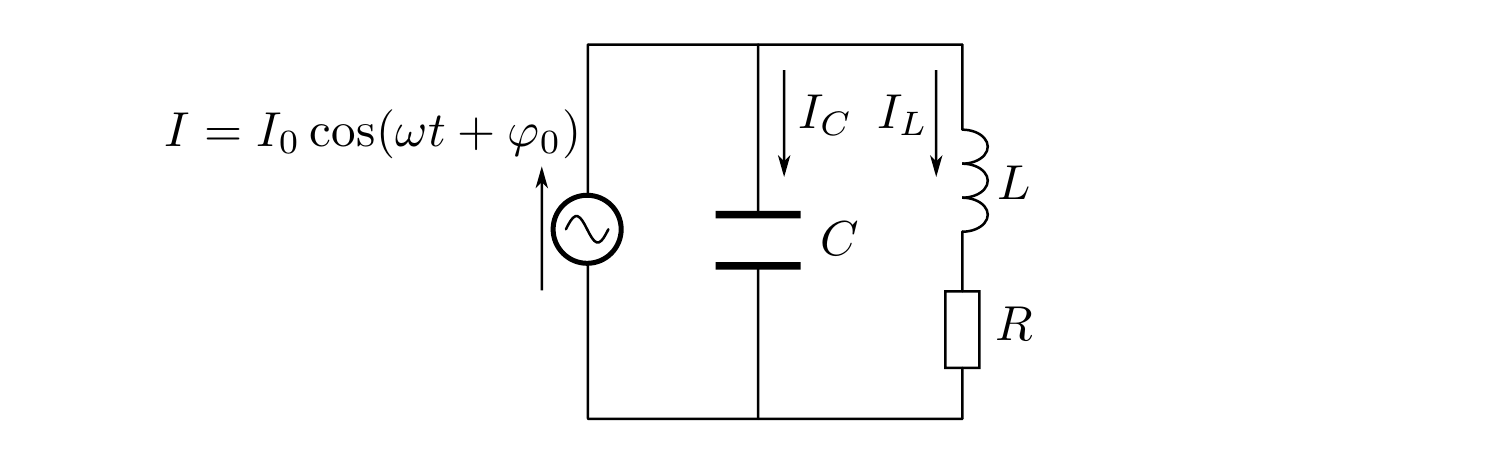
\includegraphics[scale=2]{1.png}
\end{center}
\caption{Параллельный контур с внешним гармоническим источником ЭДС}
\label{ris1}
\end{figure}

Контур подключён к источнику ЭДС, задающему во внешней цепи ток, изменяющийся по гармоническому закону: $I = I_0 \cos{(\omega t + \varphi_0)}$. Таким образом, мы предполагаем, что внутреннее сопротивлением источника столь велико, что он является генератором тока, который по определению обладает бесконечно большим внутренним сопротивлением. Потерями в катушке индуктивности и конденсаторе будем, как и ранее, пренебрегать. Необходимые уточнения будут сделаны в описаниях соответствующих лабораторных работ.

Воспользуемся формулами для импедансов элементов цепи и правилами сложения сопротивлений. Для комплексных амплитуд токов в ёмкостной $\mathbf{I_C}$ и индуктивной $\mathbf{I_L}$ ветвях контура, а также для напряжения $\mathbf{U}$ на контуре (совпадающем в нашем приближении с напряжением на конденсаторе) при нулевой начальной фазе тока $\varphi_0 = 0$ получаем выражения
\begin{align}
& \mathbf{I_C} = \mathbf{I} \frac{Z_{LR}}{Z_C + Z_{LR}} = I_0 \frac{1 + i \frac{\rho \omega}{R \omega_0}}{1 + i \frac{\rho}{R}\left(\frac{\omega}{\omega_0} - \frac{\omega_0}{\omega}\right)}, \\
& \mathbf{I_L} = \mathbf{I} \frac{Z_{C}}{Z_C + Z_{LR}} = I_0 \frac{-i \frac{\rho \omega_0}{R \omega}}{1 + i \frac{\rho}{R}\left(\frac{\omega}{\omega_0} - \frac{\omega_0}{\omega}\right)}, \label{eq:Ic IL U} \\
& \mathbf{U} = \mathbf{I} \frac{Z_C Z_{LR}}{Z_C + Z_{LR}} = I_0 \frac{\rho^2}{R} \frac{1 - i \frac{\rho \omega_0}{R \omega}}{1 + i \frac{\rho}{R}\left(\frac{\omega}{\omega_0} - \frac{\omega_0}{\omega}\right)}, \\
\end{align}
где $Z_C = \frac{1}{i \omega C}$ и $Z_{LR} = R + i \omega L$ --- импедансы ёмкостной и индуктивной ветвей параллельного контура соответственно.

Ограничимся рассмотрением наиболее интересного случая контура с
высокой добротностью вблизи резонансной частоты, когда $Q\approx \rho / R \gg 1$,
выполняется условие и применимо разложение. При этом
вещественные части комплексных амплитуд \eqref{eq:Ic IL U} можно представить
в виде
\begin{align}
& I_C(t) = Q I_0 \frac{\omega}{\omega_0} \frac{\cos{(\omega t - \psi_C)}}{\sqrt{1 + (\tau \Delta{\omega})^2}}, & &\psi_C = \arctan{(\tau \Delta{\omega})} - \frac{\pi}{2} + \frac{1}{Q}, \\
& I_L(t) = Q I_0 \frac{\omega_0}{\omega} \frac{\cos{(\omega t - \psi_L)}}{\sqrt{1 + (\tau \Delta{\omega})^2}}, & &\psi_L = \arctan{(\tau \Delta{\omega})} + \frac{\pi}{2}, \label{eq:Ic IL U (t)} \\
& U(t) = Q \rho I_0 \frac{\cos{(\omega t - \psi_U)}}{\sqrt{1 + (\tau \Delta{\omega})^2}}, & &\psi_U = \arctan{(\tau \Delta{\omega})} + \frac{\omega_0}{\omega} \frac{1}{Q}. \\
\end{align}

При резонансе, когда в принятом выше приближении $\omega = \omega_0$, $\Delta{\omega} = 0$, амплитуды токов в ветвях контура, напряжения на нём, фазовые сдвиги $\psi$ и их производные по циклической частоте $\psi' = d\psi/d\omega$ принимают вид
\begin{align}
& I_{C_{\omega}}(\omega_0) = Q I_0, & &\psi_C(\omega_0) = - \frac{\pi}{2} + \frac{1}{Q}, \\
& I_{L_{\omega}}(\omega_0) = Q I_0, & &\psi_L(\omega_0) = \frac{\pi}{2}, \label{eq:Ic IL U (w)} \\
& U_{\omega}(\omega_0) = Q^2 R I_0, & &\psi_U(\omega_0) = \frac{1}{Q}. \\
\end{align}
\begin{equation}\label{eq:psi C L U}
\psi'_C(\omega_0) = \psi'_L(\omega_0) = \psi'_U(\omega_0) = \tau.
\end{equation}
Из формул \eqref{eq:Ic IL U (w)} следует, что на частоте $\omega_0$ токи $I_C$ и $I_L$ в ёмкостной и индуктивной ветвях контура в $Q$ раз превышают ток $I$ во внешней цепи. При этом ток $I_C$ опережает внешний ток $I$ по фазе почти на $\pi/2$,а ток $I_L$ — отстаёт на $\pi/2$. Между собой токи $I_C$ и $I_L$ сдвинуты по фазе на угол, близкий к $\pi$. Можно сказать, что токи $I_C$ и $I_L$ образуют контурный ток, последовательно обтекающий элементы контура и в $Q$ раз превышающий по амплитуде внешний ток $I$. Последнее обстоятельство послужило поводом назвать резонанс в параллельном контуре резонансом токов.

Отметим, однако, что максимальные значения токов в контуре не строго равны $Q I_0$ и достигаются не строго на частоте $\omega_0$. Соответствующие относительные поправки, как и в случае резонанса напряжения, обусловлены входящими в выражения \eqref{eq:Ic IL U (t)} для токов $I_C$ , $I_L$ множителями $(\omega_0 / \omega)^{\pm 1}$ и составляют доли малой величины $Q^{-2}$.

Из формул \eqref{eq:Ic IL U} вытекает, что на частоте $\omega_0$ импеданс контура $Z(\omega_0) = U(\omega_0)/I_0$ является почти чисто активным. В пренебрежении малыми поправками порядка $Q^{-2}$ его модуль и фаза относительно внешнего тока соответственно равны:
\begin{equation}\label{eq:Z(w)}
|Z(\omega_0)| = Q^2 R, \quad \psi_Z(\omega_0) = \frac{1}{Q}.
\end{equation}

Как видим, сопротивление контура в резонансе в $Q^2$ раз превышает его активное сопротивление $R$. Это свойство параллельного контура широко используется в радиотехнике.

По формулам \eqref{eq:Ic IL U (w)} легко построить векторную диаграмму для резонанса токов в рассмотренном выше параллельном контуре, в котором не учитывались потери в конденсаторе и катушке индуктивности. Подобная диаграмма показана на рис.~\ref{ris2}.

\begin{figure}[h!]
\begin{center}
    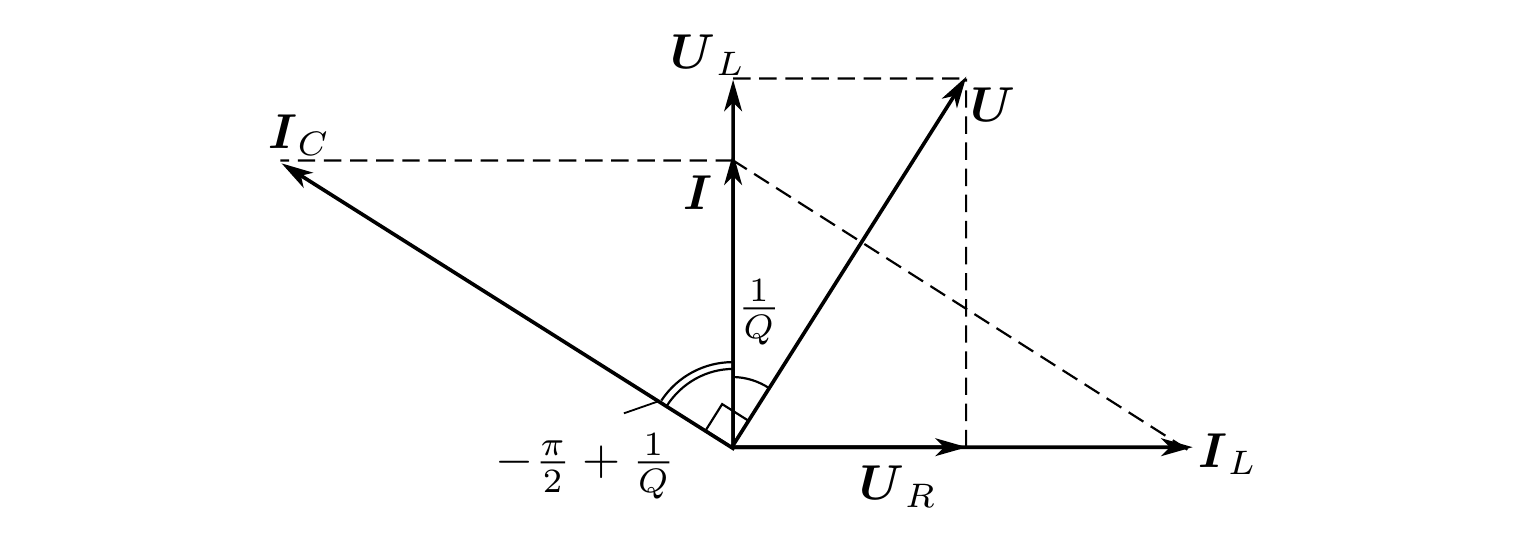
\includegraphics[scale=2]{2.png}
\end{center}
\caption{Векторная диаграмма при резонансе токов}
\label{ris2}
\end{figure}

По оси ординат диаграммы отложен внешний ток $\mathbf{I}$. Напряжение на конденсаторе, равное напряжению на контуре $\mathbf{U}$, с учётом принятого правила знаков отстаёт по фазе от тока $\mathbf{I}$ на угол $Q^{-1}$. Ток $\mathbf{I_C}$ через конденсатор (без потерь) опережает по фазе напряжение $U$ на $\pi/2$. Ток через индуктивность $\mathbf{I_L}$ отстаёт от внешнего тока $I$ по фазе на $\pi/2$.

Напряжение $\mathbf{U_R}$ на сопротивлении совпадает по фазе с током $\mathbf{I_L}$, напряжение $\mathbf{U_L}$ на индуктивности (без потерь) опережает ток $\mathbf{I_L}$ на $\pi/2$. Как видим, контур с активными потерями только в индуктивной ветви проявляет ёмкостную реакцию: напряжение на контуре отстаёт по фазе от тока.

Таким образом, условия резонанса токов в параллельном контуре и резонанса напряжений в последовательном высокодобротном контуре совпадают: $\omega = \omega_0$. Но если в последовательном контуре резонансное сопротивление контура равно чисто активному сопротивлению цепи $R$ и минимально, обеспечивая максимум тока при заданном внешнем напряжении, то в параллельном контуре резонансное сопротивление контура почти чисто активное, обратно пропорционально $R$ и в $Q^2$ раз его превышает, обеспечивая максимум напряжения на контуре при заданном внешнем токе. Сдвиг фаз между напряжением и током при резонансе напряжений всегда отсутствует, а при резонансе токов он близок к нулю, только если $Q \gg 1$.

\section{Методика измерений}

\begin{figure}[h!]
\begin{center}
    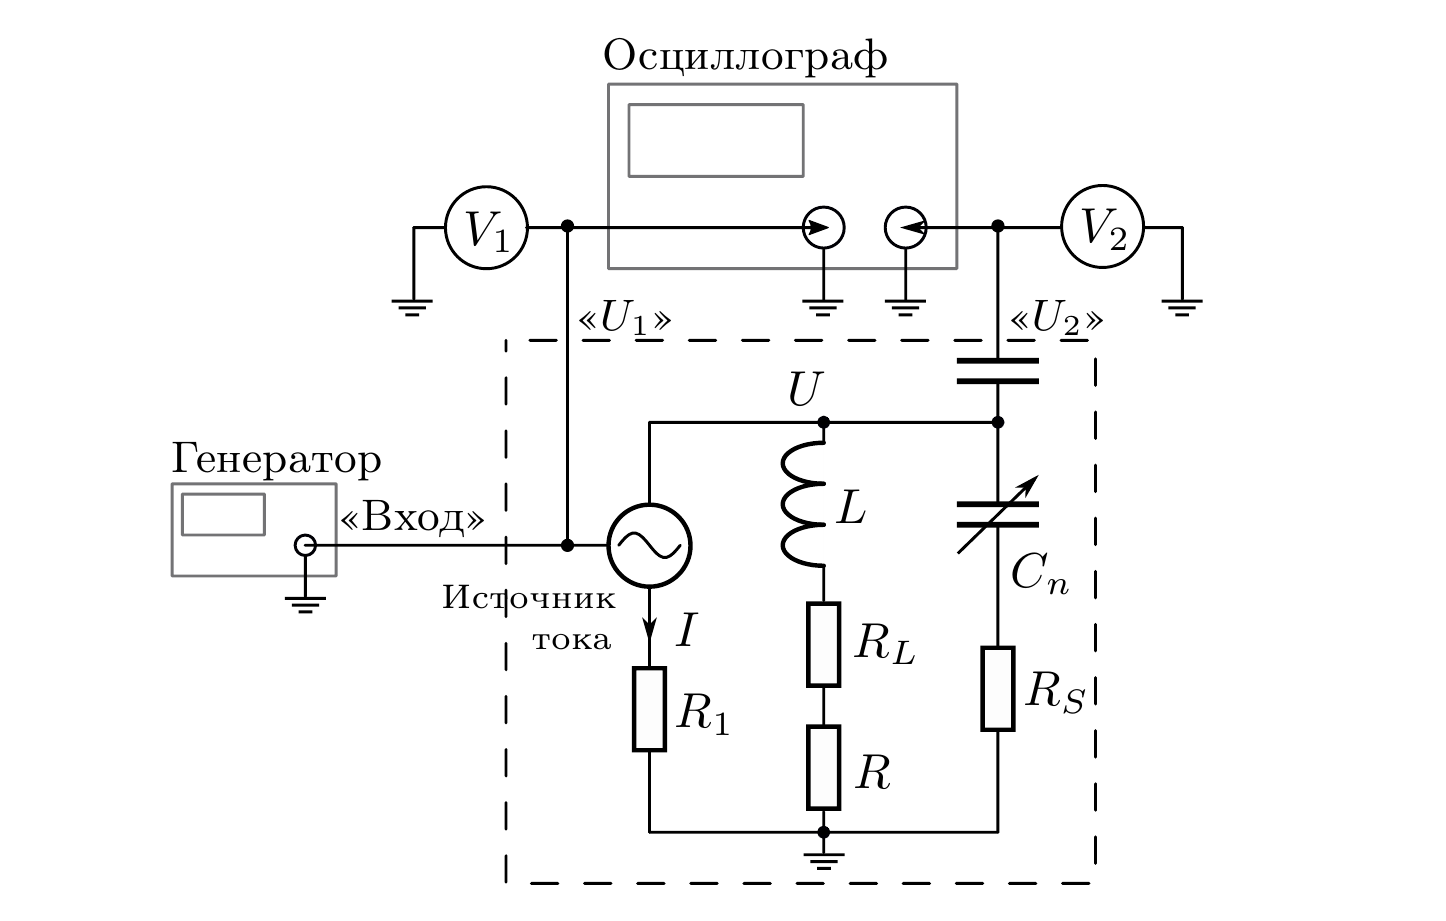
\includegraphics[scale=2.5]{ust.png}
\end{center}
\caption{Блок-схема экспериментального стенда}
\label{ust}
\end{figure}

$I=\dfrac{E}{R_I}=\dfrac{E_0cos(\omega t+\varphi_0)}{R_I}=I_0cos(\omega t+\varphi_0)$ --- ток на генераторе.

\begin{equation}\label{eq:Rs}
R_S=\dfrac{U_{RS}}{I}=\frac{U_{RS}}{\omega CU_{CS}}=\dfrac{1}{\omega C}tg\delta,
\end{equation}
где $R_S$ --- эквивалентное последовательное сопротивление (ЭПС).

Для используемых емкостей $C_n$ выполнено $tg\delta<10^{-3}$.

\begin{equation}\label{eq:Rsum}
R_{\sum}=R+R_L+R_S,
\end{equation}
где $R_{\sum}$ --- суммарное активное сопротивление контура.

Воспользуемся методом комплексных амплитуд:
$$Z_L=R_L+i\omega L, \quad Z_C=R_S-i\frac{1}{\omega C}, \quad Z=R_{\sum}+i(\omega L-\dfrac{1}{\omega C}).$$

Тогда напряжение на контуре и токи на индуктивной и емкостной частях контура при нулевой начальной фазе можно представить в виде:
$$I_c=I\dfrac{Z_L}{Z_C+Z_L}=iQI_0\dfrac{\omega}{\omega_0}\dfrac{1-i\dfrac{R+R_L}{\rho}\dfrac{\omega_0}{\omega}}{1+iQ(\dfrac{\omega}{\omega_0}-\dfrac{\omega_0}{\omega})},$$
$$I_L=I\dfrac{Z_c}{Z_C+Z_L}=iQI_0\frac{\omega_0}{\omega}\frac{1+itg\delta}{1+iQ(\frac{\omega}{\omega_0}-\frac{\omega_0}{\omega})},$$
$$U=I\frac{Z_LZ_c}{Z_C+Z_L}=Q\rho I_0\frac{(1-i\frac{R+R_L}{\rho}\frac{\omega_0}{\omega})(1+itg\delta)}{1+iQ(\frac{\omega}{\omega_0}-\frac{\omega_0}{\omega})},$$
где $\omega_0=\frac{1}{\sqrt{LC}}$ --- собственная частота, $\rho=\sqrt{\frac{L}{C}}$ --- реактивное сопротивление контура, $Q=\frac{\rho}{R_{\sum}}$ --- добротность контура.

Рассмотрим случай, когда $|\Delta\omega|=|\omega-\omega_0|\ll\omega_0$. Тогда
$$\frac{\omega}{\omega_0}-\frac{\omega_0}{\omega}=\frac{2\Delta\omega}{\omega_0}.$$
Пренебрегая поправками порядка $Q^{-2}$, получим:
$$I_c=QI_0\frac{\omega}{\omega_0}\frac{e^{i\phi_c}}{\sqrt{1+(\tau\Delta\omega)^2}}, \quad \phi_c=\frac{\pi}{2}-\frac{R+R_L}{\rho}-arctg(\tau\Delta\omega),$$
$$I_L=QI_0\frac{\omega_0}{\omega}\frac{e^{i\phi_L}}{\sqrt{1+(\tau\Delta\omega)^2}}, \quad \phi_L=-\frac{\pi}{2}+\delta\arctg(\tau\Delta\omega),$$
$$U=Q\rho I_0\frac{\omega}{\omega_0}\frac{e^{i\phi_U}}{\sqrt{1+(\tau\Delta\omega)^2}}, \quad \phi_U=-\frac{\omega}{\omega_0}\frac{R+R_L}{\rho}+\delta-arctg(\tau\Delta\omega),$$
где $\tau=\frac{2L}{R_{\sum}}=\frac{2Q}{\omega_0}$ --- время затухания.

При резонансе, т. е. когда $\Delta\omega=0$:
$$I_c(\omega_0)=QI_0, \quad \phi_c(\omega_0)=\frac{\pi}{2}-\frac{R+R_L}{\rho},$$
$$I_L(\omega_0)=QI_0, \quad \phi_L(\omega_0)=-\frac{\pi}{2}+\delta,$$
$$U(\omega_0)=Q\rho I_0=Q^2R_{\sum}I_0, \quad \phi_U{\omega_0}=-\frac{R+R_L}{\rho}+\delta,$$
$$\phi'_c(\omega_0)=\phi'_L(\omega_0)=\phi'_U(\omega_0)=-\tau.$$
  	
\section{Используемое оборудование}

\begin{enumerate}
    \item генератор сигналов;
    \item источник напряжения;
    \item двухканальный осциллограф;
    \item цифровые вольтметры;
\end{enumerate}

\section{Результаты измерений и обработка данных}

Параметры установки:
\begin{description}
\item{} $R = 3,5~Ом$
\item{} $R_1 = 1008~Ом$
\end{description}

Получим формулы для вычисления параметров контура:
\begin{equation}
\omega_0 = 2\pi f = \frac{1}{\sqrt{L C}} \Rightarrow L = \frac{1}{C(2\pi f)^2},
\end{equation}
\begin{equation}
\rho \triangleq \sqrt{\frac{L}{C}} \Rightarrow \rho = \frac{1}{2\pi fC},
\end{equation}
\begin{equation}
I_0 = \frac{E_0}{R_1} \Rightarrow Z_{\text{рез}} = \frac{U}{I_0} = \frac{U}{E_0}R_1.
\end{equation}
Из формул~\eqref{eq:Ic IL U (w)} следует:
\begin{equation}
Z_{рез} = Q \rho \Rightarrow Q = \frac{Z_{рез}}{\rho} = \frac{UR_1}{E_0}2\pi fC,
\end{equation}
\begin{equation}
Q = \frac{\rho}{R_{\sum}} \Rightarrow R_{\sum} = \frac{\rho}{Q} = \frac{E_0}{UR_1}\frac{1}{(2\pi fC)^2}.
\end{equation}
Из формулы \eqref{eq:Rs} (при максимальном значении $\mathrm{tg}\,\delta = 10^{-3}$) получаем:
\begin{equation}
R_{Smax} =10^{-3}\cdot\frac{1}{\omega_0C},
\end{equation}
Тогда из формулы \eqref{eq:Rsum} находим:
\begin{equation}
R_L = R_{sum} - R - R_S = \frac{E_0}{UR_1}\frac{1}{(2\pi fC)^2}-R-10^{-3}\cdot\frac{1}{\omega_0C}.
\end{equation}

Результаты измерения резонансных частот для 7 разных конденсаторов и вычисления параметров контура представлены в таб.~\ref{tab1}. 

\begin{table}[h!]
\begin{center}
\begin{tabular}{|cccc|c|c|c|c|c|c|c|}
\hline
\multicolumn{1}{|c|}{$С, нФ$} & \multicolumn{1}{c|}{$f, кГц$} & \multicolumn{1}{c|}{$U, B$}  & $E, B$  & $L, мкГн$ & $\rho, Ом$ & $|Z_{рез}|, Ом$ & $Q$  & $R_{\sum}, Ом$ & $R_{S_{max}}, Ом$ & $R_L, Ом$ \\ \hline
\multicolumn{1}{|c|}{25,1}  & \multicolumn{1}{c|}{32,12}  & \multicolumn{1}{c|}{1,190} & 0,202 & 978,2   & 197,4   & 5938,2     & 30 & 6,56     & 0,20      & 2,87     \\ \hline
\multicolumn{1}{|c|}{33,2}  & \multicolumn{1}{c|}{27,79}  & \multicolumn{1}{c|}{0,790} & 0,202 & 987,9   & 172,5   & 3942,2     & 23 & 7,55     & 0,17      & 3,88     \\ \hline
\multicolumn{1}{|c|}{47,3}  & \multicolumn{1}{c|}{23,16}  & \multicolumn{1}{c|}{0,670} & 0,202 & 998,4   & 145,3   & 3343,4     & 23 & 6,31     & 0,15      & 2,67     \\ \hline
\multicolumn{1}{|c|}{57,4}  & \multicolumn{1}{c|}{21,28}  & \multicolumn{1}{c|}{0,573} & 0,202 & 974,5   & 130,3   & 2859,3     & 22 & 5,94     & 0,13      & 2,31     \\ \hline
\multicolumn{1}{|c|}{67,5}  & \multicolumn{1}{c|}{19,46}  & \multicolumn{1}{c|}{0,449} & 0,202 & 990,9   & 121,2   & 2240,6     & 18 & 6,55     & 0,12      & 2,93     \\ \hline
\multicolumn{1}{|c|}{82,7}  & \multicolumn{1}{c|}{17,67}  & \multicolumn{1}{c|}{0,380} & 0,202 & 981,0   & 108,9   & 1896,2     & 17 & 6,26     & 0,11      & 2,65     \\ \hline
\multicolumn{1}{|c|}{101,6} & \multicolumn{1}{c|}{16,02}  & \multicolumn{1}{c|}{0,335} & 0,202 & 971,5   & 97,8    & 1671,7     & 17 & 5,72     & 0,10      & 2,12     \\ \hline
\multicolumn{4}{|c|}{Среднее значение}                                                         & 983,2   &         &            &    &          &           & 2,77     \\ \hline
\multicolumn{4}{|c|}{Случ. погрешность}                                                        & 3,6     &         &            &    &          &           & 0,21     \\ \hline
\end{tabular}
\end{center}
\caption{Параметры колебательного контура при разных значениях ёмкости конденсатора}
\label{tab1}
\end{table}

Результаты измерений амплитудно-частотной характеристики $U(\nu)$ для 1-ой ($25,1~нФ$) и 7-ой ($101,6~нФ$) ёмкостей конденсатора представлены в таб.~\ref{tab2}~и~\ref{tab3}.

\begin{table}[h!]
\begin{center}
\begin{tabular}{|c|c|c|c|}
\hline
$\nu, кГц$ & $\delta_{\nu}, кГц$ & $U, B$  & $\delta_U, B$ \\ \hline
31,38  & 0,01    & 0,682 & 0,001 \\ \hline
31,44  & 0,01    & 0,715 & 0,001 \\ \hline
31,51  & 0,01    & 0,765 & 0,001 \\ \hline
31,58  & 0,01    & 0,822 & 0,001 \\ \hline
31,69  & 0,01    & 0,910 & 0,001 \\ \hline
31,73  & 0,01    & 0,951 & 0,001 \\ \hline
31,78  & 0,01    & 0,992 & 0,001 \\ \hline
32,08  & 0,01    & 1,187 & 0,001 \\ \hline
32,86  & 0,01    & 0,705 & 0,001 \\ \hline
32,81  & 0,01    & 0,735 & 0,001 \\ \hline
32,68  & 0,01    & 0,825 & 0,001 \\ \hline
32,48  & 0,01    & 0,986 & 0,001 \\ \hline
32,30  & 0,01    & 1,127 & 0,001 \\ \hline
32,12  & 0,01    & 1,189 & 0,001 \\ \hline
\end{tabular}
\end{center}
\caption{Амплитудно-частотная характеристика колебательного контура для 1-ой ёмкости}
\label{tab2}
\end{table}

\begin{table}[h!]
\begin{center}
\begin{tabular}{|c|c|c|c|}
\hline
$\nu, кГц$ & $\delta_{\nu}, кГц$ & $U, B$  & $\delta_U, B$ \\ \hline
15,41  & 0,01    & 0,193 & 0,001 \\ \hline
15,51  & 0,01    & 0,215 & 0,001 \\ \hline
15,54  & 0,01    & 0,222 & 0,001 \\ \hline
15,60  & 0,01    & 0,239 & 0,001 \\ \hline
15,61  & 0,01    & 0,242 & 0,001 \\ \hline
15,64  & 0,01    & 0,250 & 0,001 \\ \hline
15,69  & 0,01    & 0,267 & 0,001 \\ \hline
15,78  & 0,01    & 0,289 & 0,001 \\ \hline
15,83  & 0,01    & 0,304 & 0,001 \\ \hline
15,92  & 0,01    & 0,325 & 0,001 \\ \hline
16,03  & 0,01    & 0,338 & 0,001 \\ \hline
16,71  & 0,01    & 0,200 & 0,001 \\ \hline
16,66  & 0,01    & 0,211 & 0,001 \\ \hline
16,60  & 0,01    & 0,223 & 0,001 \\ \hline
16,52  & 0,01    & 0,243 & 0,001 \\ \hline
16,44  & 0,01    & 0,264 & 0,001 \\ \hline
16,30  & 0,01    & 0,301 & 0,001 \\ \hline
16,15  & 0,01    & 0,332 & 0,001 \\ \hline
\end{tabular}
\end{center}
\caption{Амплитудно-частотная характеристика колебательного контура для 7-ой ёмкости}
\label{tab3}
\end{table}

График амплитудно-частотных характеристик $U(\nu)$ для обеих ёмкостей представлен на рис.~\ref{plot1}.

\begin{figure}[h!]
\begin{center}
    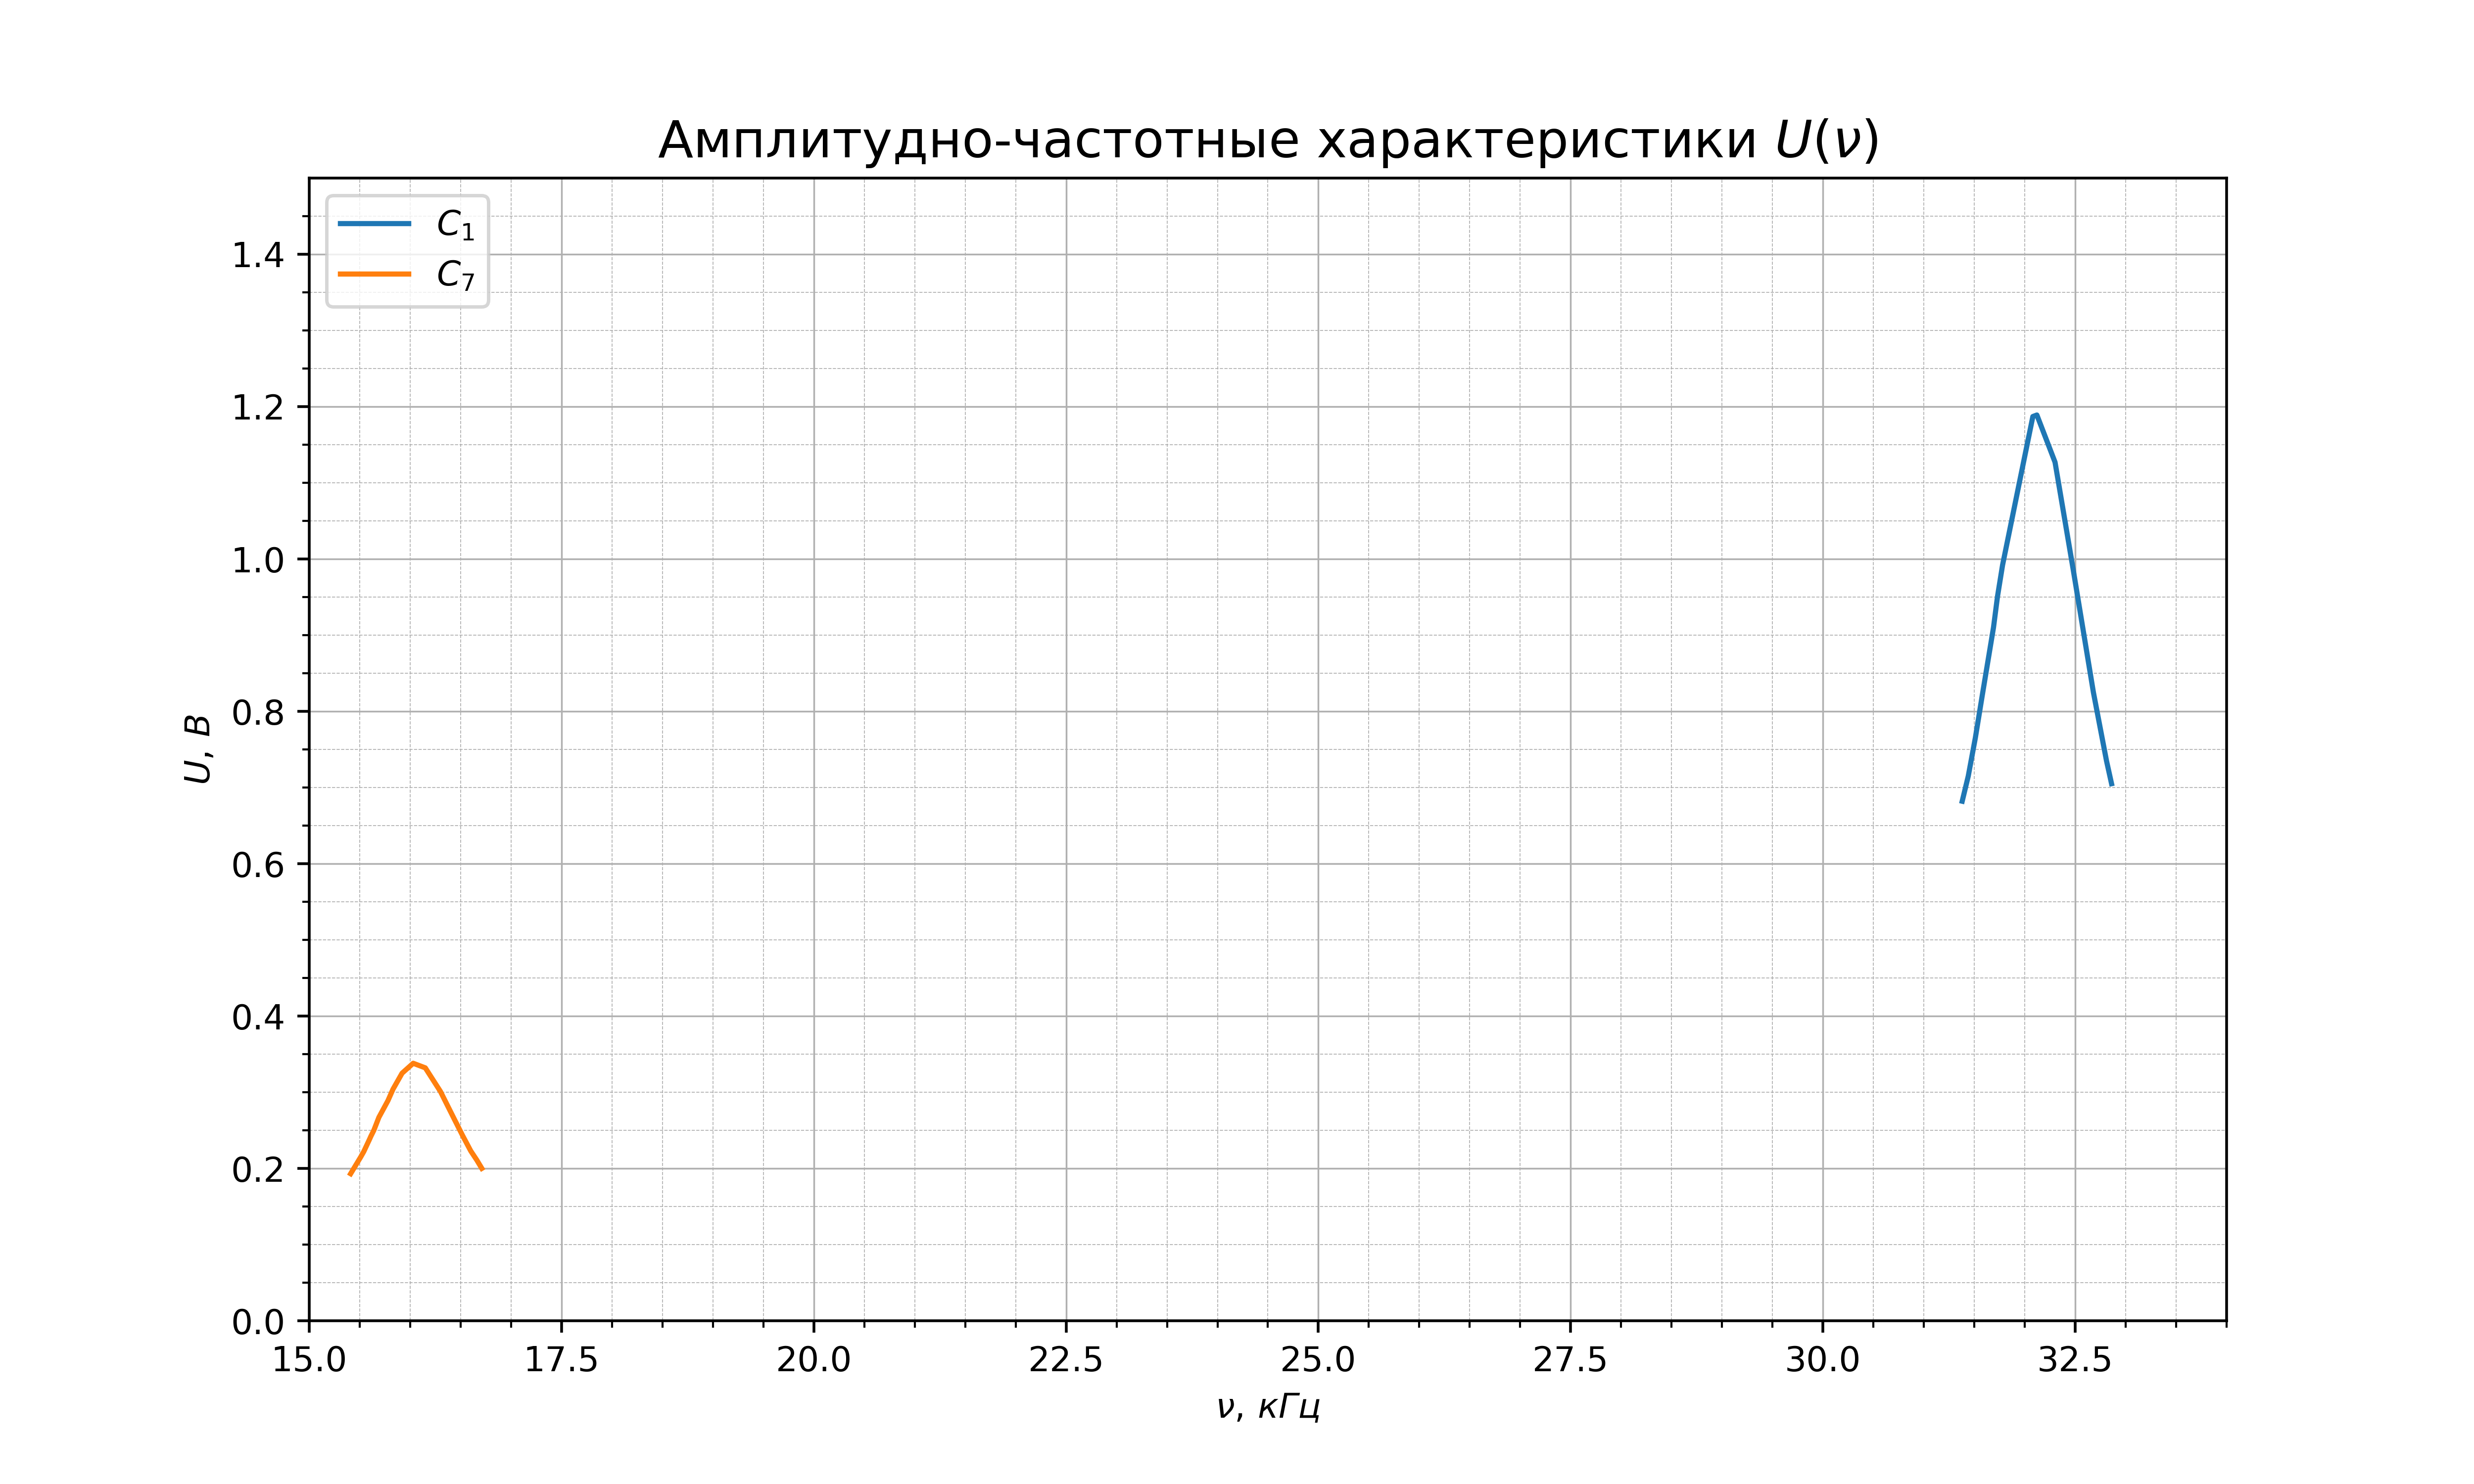
\includegraphics[scale=0.7]{3.2.3_1.png}
\end{center}
\caption{Амплитудно-частотная характеристика $U(\nu)$ для колебательного контура с 1-ой и 7-ой ёмкостями конденсатора}
\label{plot1}
\end{figure}

\newpage

График амплитудно-частотных характеристик $U(\nu)$ для обеих ёмкостей в безразмерных координатах представлен на рис.~\ref{plot2}. Кривая для ёмкости $C_7$ шире, чем для ёмкости $C_1$, что говорит о меньшей добротности контура с ёмкостью $C_7$.

\begin{figure}[h!]
\begin{center}
    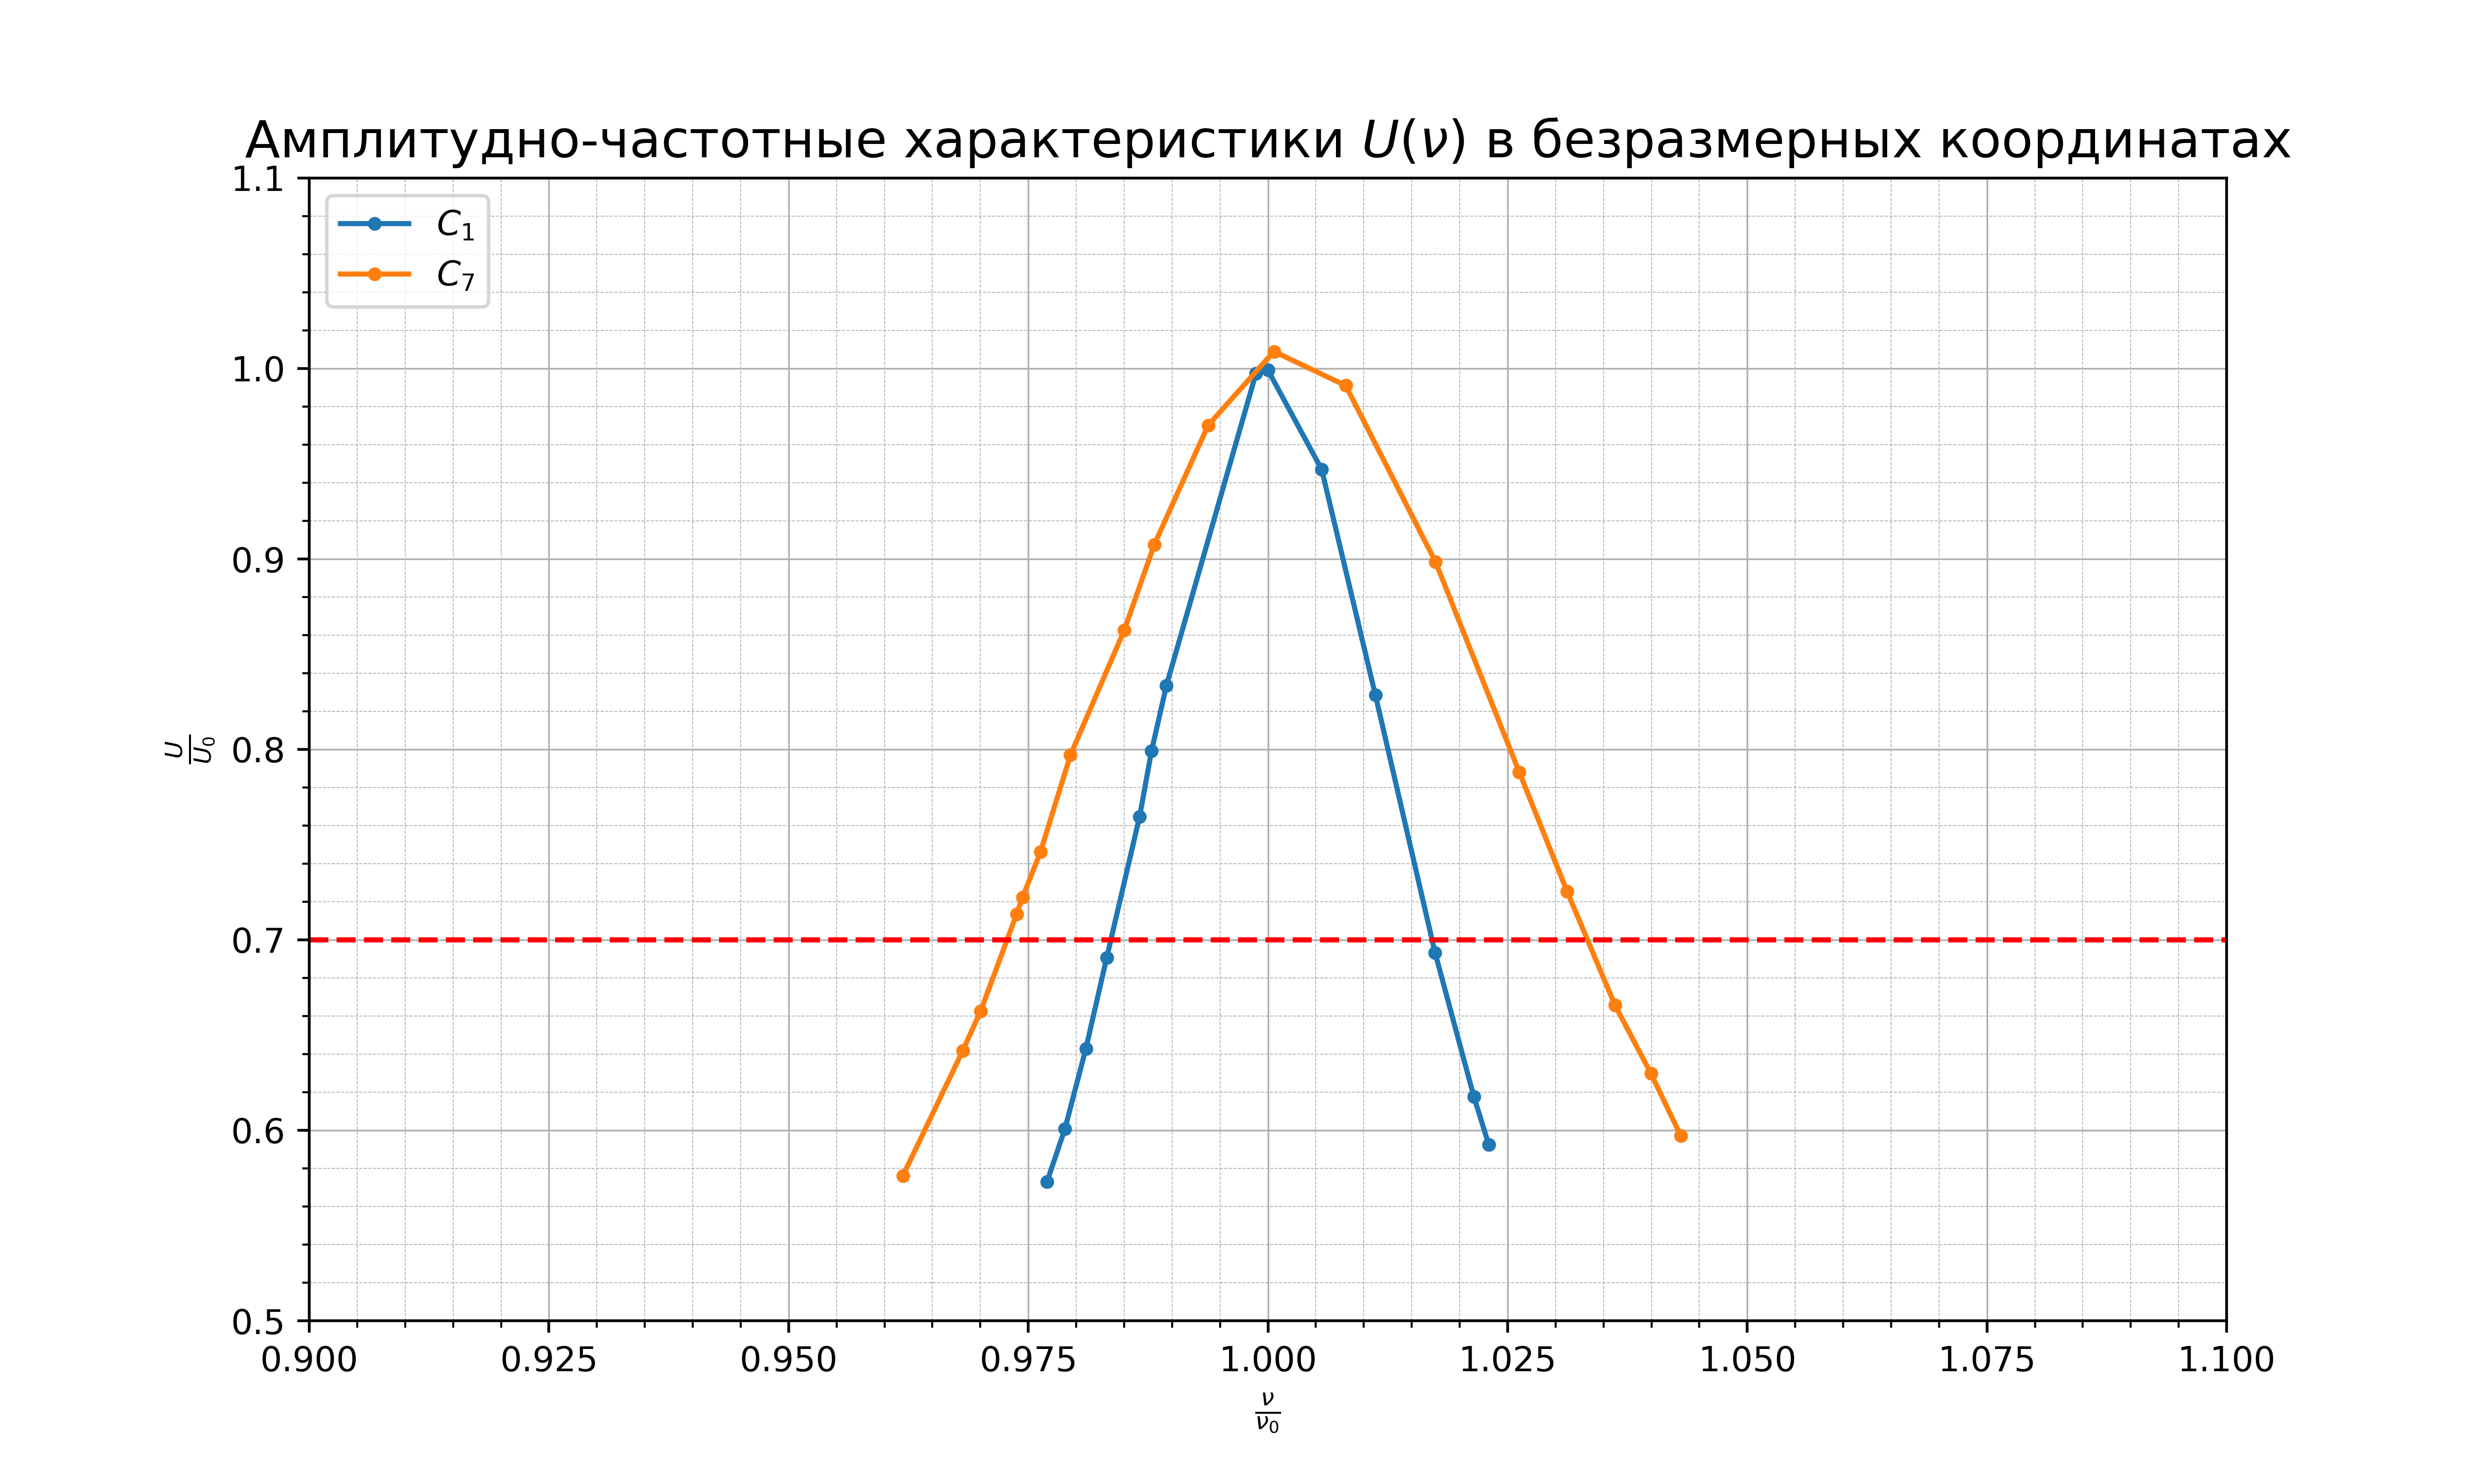
\includegraphics[scale=0.7]{3.2.3_2.png}
\end{center}
\caption{Амплитудно-частотная характеристика $U(\nu)$ для колебательного контура с 1-ой и 7-ой ёмкостями конденсатора в безразмерных координатах}
\label{plot2}
\end{figure}

Добротность определяется по формуле $Q = \frac{1}{\delta \omega}$, где $\delta \omega$ --- ширина резонансных кривых на уровне $\frac{1}{\sqrt{2}} = 0,707$. Полученные значения добротности:
$$ Q_1 = 29\pm1, \quad Q_7 = 16\pm1.$$

\newpage

Результаты измерений фазово-частотной характеристики $\psi_U(\nu)$ для 1-ой и 7-ой ёмкостей конденсатора представлены в таб.~\ref{tab4}~и~\ref{tab5}.

\begin{table}[h!]
\begin{center}
\begin{tabular}{|c|c|c|c|c|c|c|c|c|}
\hline
$\nu, кГц$ & $\delta_{\nu}, кГц$ & знак $\psi_U$ & $x, дел$ & $\delta_x, дел$ & $x_0, дел$ & $\delta_{x_0}, дел$ & $\psi_U, \pi \cdot рад$ & $\delta_{\psi_U}, \pi \cdot рад$ \\ \hline
30,35  & 0,01    & -1         & 3,5    & 0,5     & 17,0    & 0,5      & -0,21        & 0,03           \\ \hline
30,75  & 0,01    & -1         & 3,5    & 0,5     & 17,0    & 0,5      & -0,21        & 0,03           \\ \hline
30,99  & 0,01    & -1         & 3,0    & 0,5     & 16,5    & 0,5      & -0,18        & 0,03           \\ \hline
31,10  & 0,01    & -1         & 3,0    & 0,5     & 16,5    & 0,5      & -0,18        & 0,03           \\ \hline
31,35  & 0,01    & -1         & 3,0    & 0,5     & 16,0    & 0,5      & -0,19        & 0,03           \\ \hline
31,56  & 0,01    & -1         & 2,0    & 0,5     & 16,0    & 0,5      & -0,13        & 0,03           \\ \hline
31,64  & 0,01    & -1         & 2,0    & 0,5     & 16,0    & 0,5      & -0,13        & 0,03           \\ \hline
31,88  & 0,01    & -1         & 0,5    & 0,5     & 16,0    & 0,5      & -0,03        & 0,03           \\ \hline
32,17  & 0,01    & 1          & 0,5    & 0,5     & 16,0    & 0,5      & 0,03         & 0,03            \\ \hline
32,50  & 0,01    & 1          & 3,0    & 0,5     & 16,0    & 0,5      & 0,19         & 0,03            \\ \hline
32,68  & 0,01    & 1          & 4,0    & 0,5     & 16,0    & 0,5      & 0,25         & 0,03            \\ \hline
32,81  & 0,01    & 1          & 4,5    & 0,5     & 16,0    & 0,5      & 0,28         & 0,03            \\ \hline
32,99  & 0,01    & 1          & 5,0    & 0,5     & 16,0    & 0,5      & 0,31         & 0,03            \\ \hline
33,21  & 0,01    & 1          & 5,0    & 0,5     & 15,5    & 0,5      & 0,32         & 0,03            \\ \hline
33,67  & 0,01    & 1          & 5,5    & 0,5     & 15,5    & 0,5      & 0,35         & 0,03            \\ \hline
34,28  & 0,01    & 1          & 6,5    & 0,5     & 15,0    & 0,5      & 0,43         & 0,04            \\ \hline
\end{tabular}
\end{center}
\caption{Фазово-частотная характеристика колебательного контура для 1-ой ёмкости}
\label{tab4}
\end{table}

\begin{table}[h!]
\begin{center}
\begin{tabular}{|c|c|c|c|c|c|c|c|c|}
\hline
$\nu, кГц$ & $\delta_{\nu}, кГц$ & знак $\psi_U$ & $x, дел$ & $\delta_x, дел$ & $x_0, дел$ & $\delta_{x_0}, дел$ & $\psi_U, \pi \cdot рад$ & $\delta_{\psi_U}, \pi \cdot рад$ \\ \hline
14,51  & 0,01    & -1         & 4,0    & 0,5     & 17,5    & 0,5      & -0,23        & 0,03           \\ \hline
14,90  & 0,01    & -1         & 4,0    & 0,5     & 17,0    & 0,5      & -0,24        & 0,03           \\ \hline
15,17  & 0,01    & -1         & 4,0    & 0,5     & 17,0    & 0,5      & -0,24        & 0,03           \\ \hline
15,51  & 0,01    & -1         & 3,5    & 0,5     & 16,5    & 0,5      & -0,21        & 0,03           \\ \hline
15,68  & 0,01    & -1         & 2,5    & 0,5     & 16,5    & 0,5      & -0,15        & 0,03           \\ \hline
15,82  & 0,01    & -1         & 2,0    & 0,5     & 16,0    & 0,5      & -0,13        & 0,03           \\ \hline
15,95  & 0,01    & -1         & 1,0    & 0,5     & 16,0    & 0,5      & -0,06        & 0,03           \\ \hline
16,12  & 0,01    & 1          & 0,5    & 0,5     & 16,0    & 0,5      & 0,03         & 0,03            \\ \hline
16,29  & 0,01    & 1          & 2,0    & 0,5     & 16,0    & 0,5      & 0,13         & 0,03            \\ \hline
16,46  & 0,01    & 1          & 4,0    & 0,5     & 16,0    & 0,5      & 0,25         & 0,03            \\ \hline
16,69  & 0,01    & 1          & 5,0    & 0,5     & 15,5    & 0,5      & 0,32         & 0,03            \\ \hline
17,02  & 0,01    & 1          & 5,5    & 0,5     & 15,0    & 0,5      & 0,37         & 0,04            \\ \hline
17,45  & 0,01    & 1          & 6,0    & 0,5     & 15,0    & 0,5      & 0,40         & 0,04            \\ \hline
\end{tabular}
\end{center}
\caption{Фазово-частотная характеристика колебательного контура для 7-ой ёмкости}
\label{tab5}
\end{table}

График фазово-частотных характеристик $\psi_U(\nu)$ для обеих ёмкостей в безразмерных координатах представлен на рис.~\ref{plot3}.

\begin{figure}[h!]
\begin{center}
    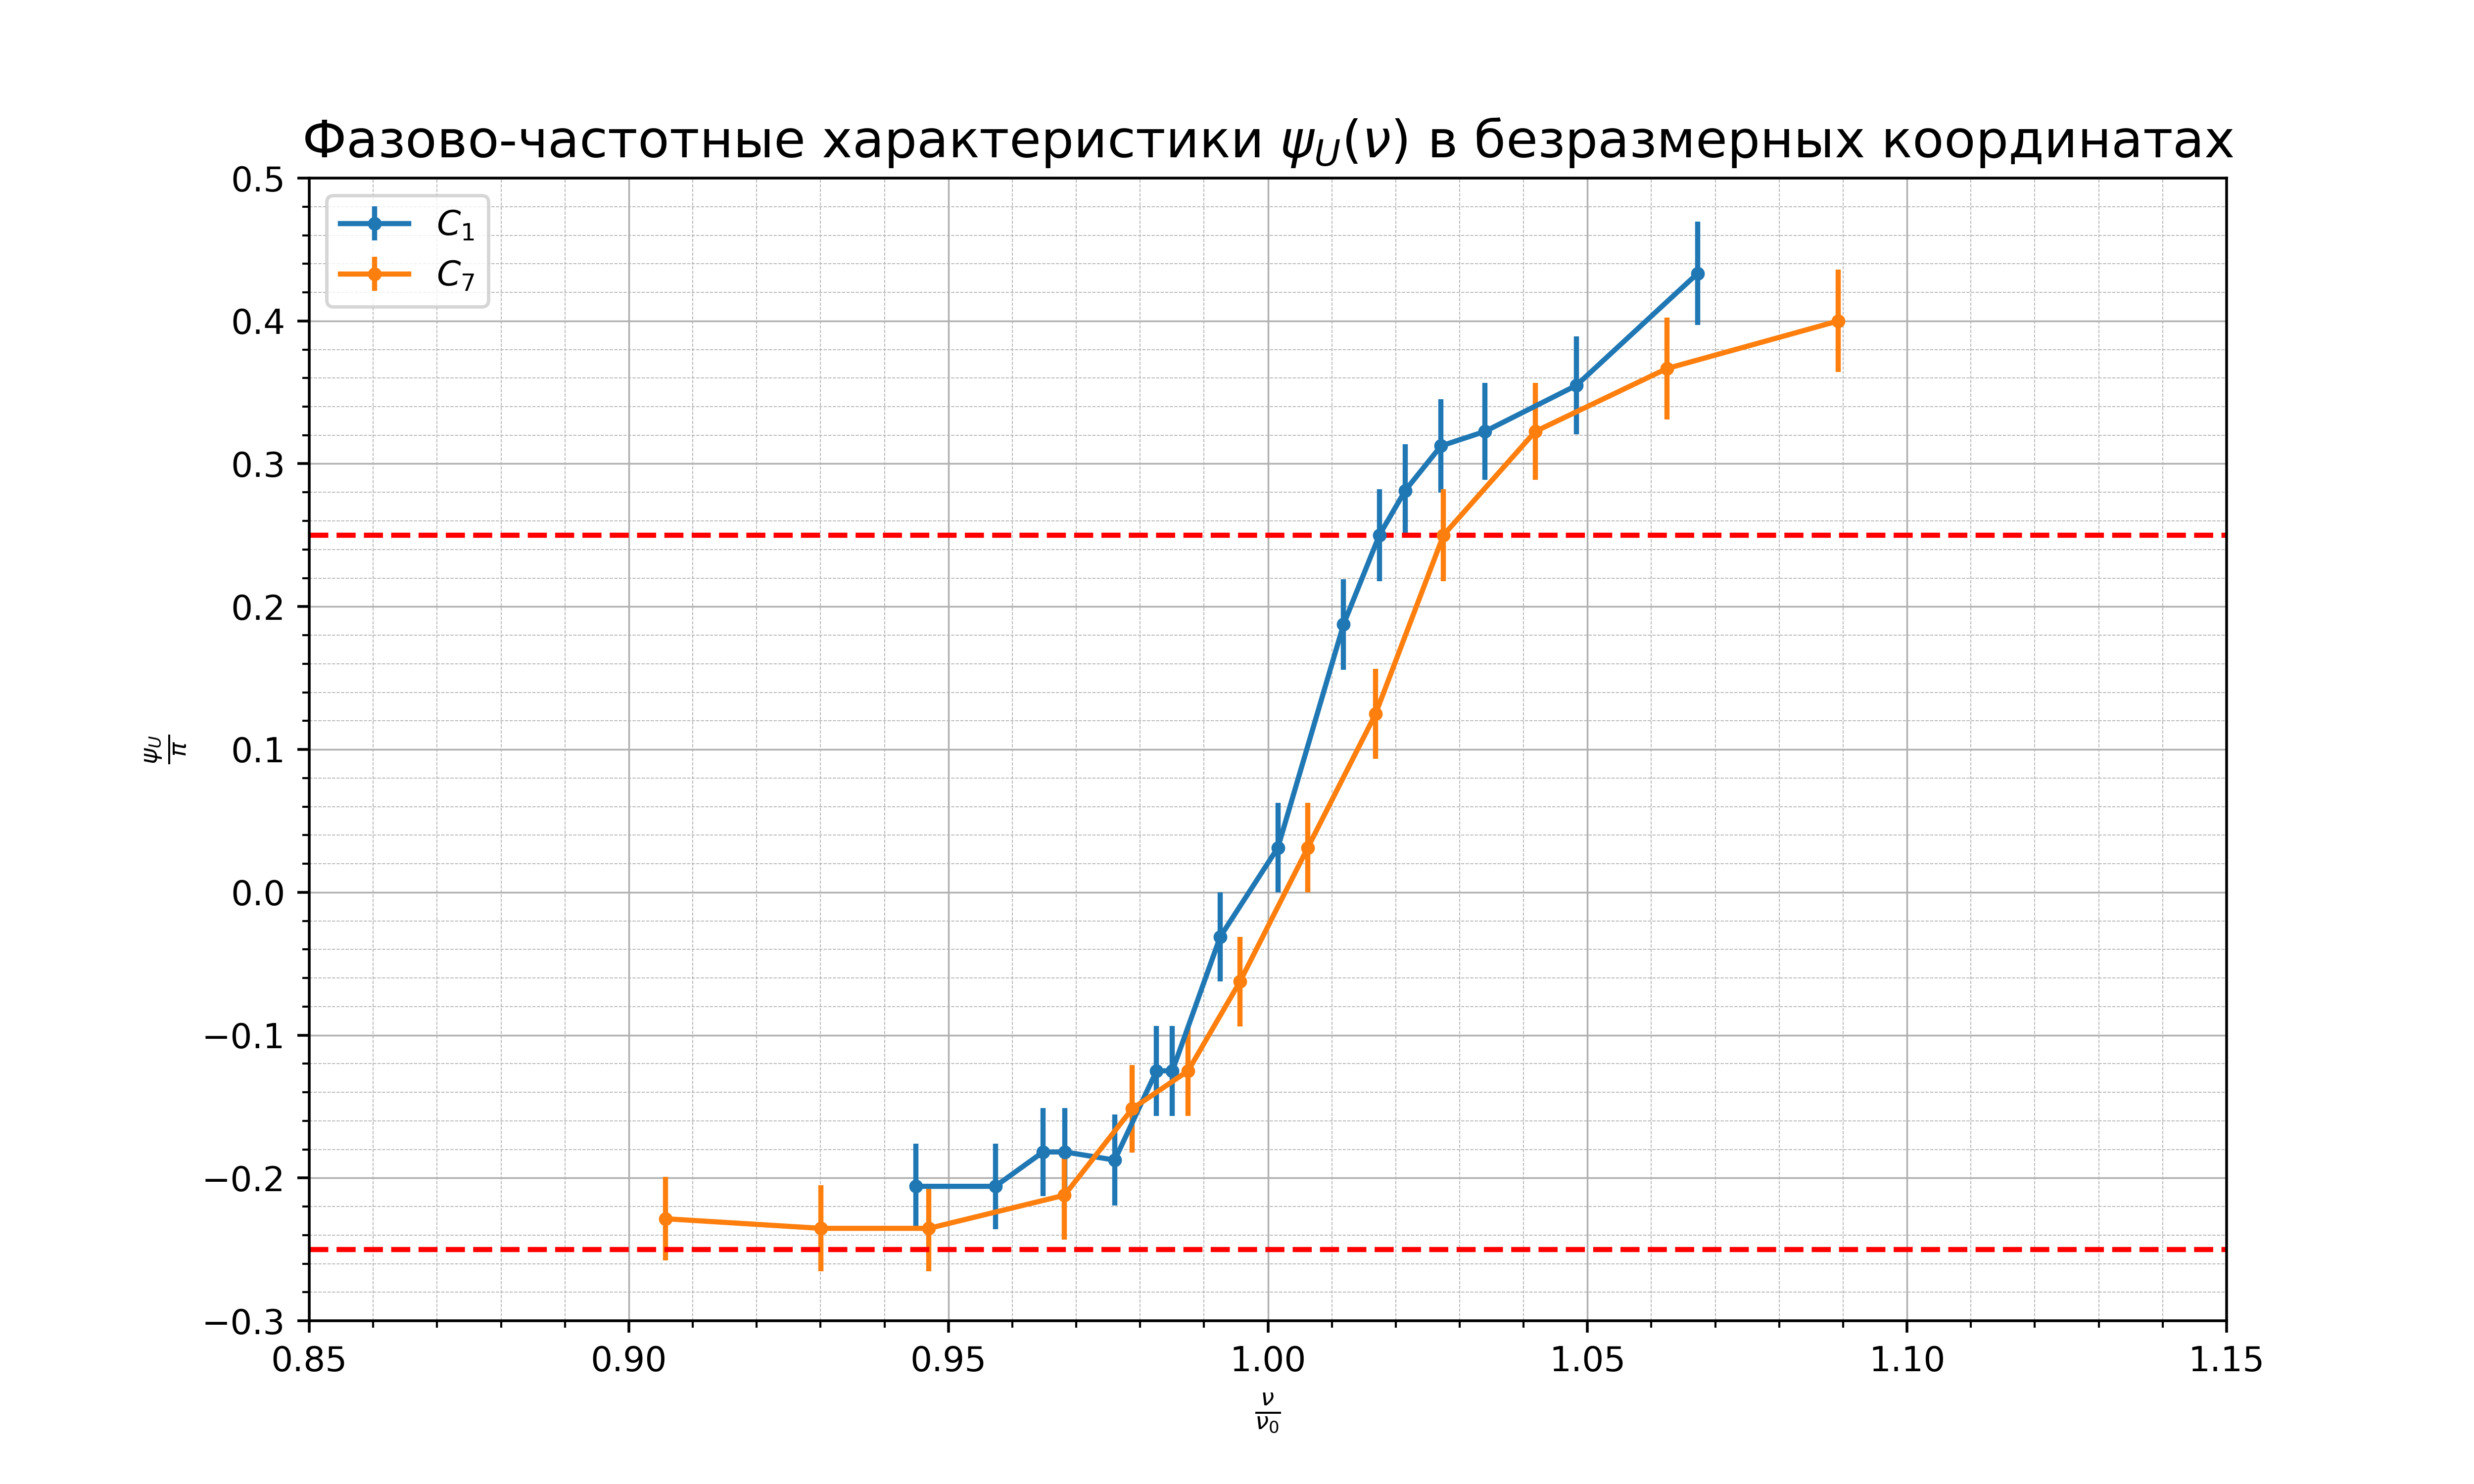
\includegraphics[scale=0.7]{3.2.3_3.png}
\end{center}
\caption{Фазово-частотная характеристика $\psi_U(\nu)$ для колебательного контура с 1-ой и 7-ой ёмкостями конденсатора в безразмерных координатах}
\label{plot3}
\end{figure}

Добротности контуров можно определить двумя способами: по формуле $Q = \frac{1}{2}\frac{d\psi_U(x)}{dx}$ при $x = 1$ или по расстоянию $1/Q$ между точками оси х, в которых y меняется от -1/4 до 1/4. Результаты измерения добротности 1-ым способом:
$$ Q_1 = 18\pm5, \quad Q_7 = 13\pm4.$$
Результаты измерения добротности 2-ым способом (так как график не доходит до -1/4, то были взяты значения, наиболее близкие к -1/4):
$$ Q_1 = 17\pm1, \quad Q_7 = 13\pm1.$$

График зависимости $R_L(\nu_{0n})$ представлен на рис.~\ref{plot4}.

\begin{figure}[h!]
\begin{center}
    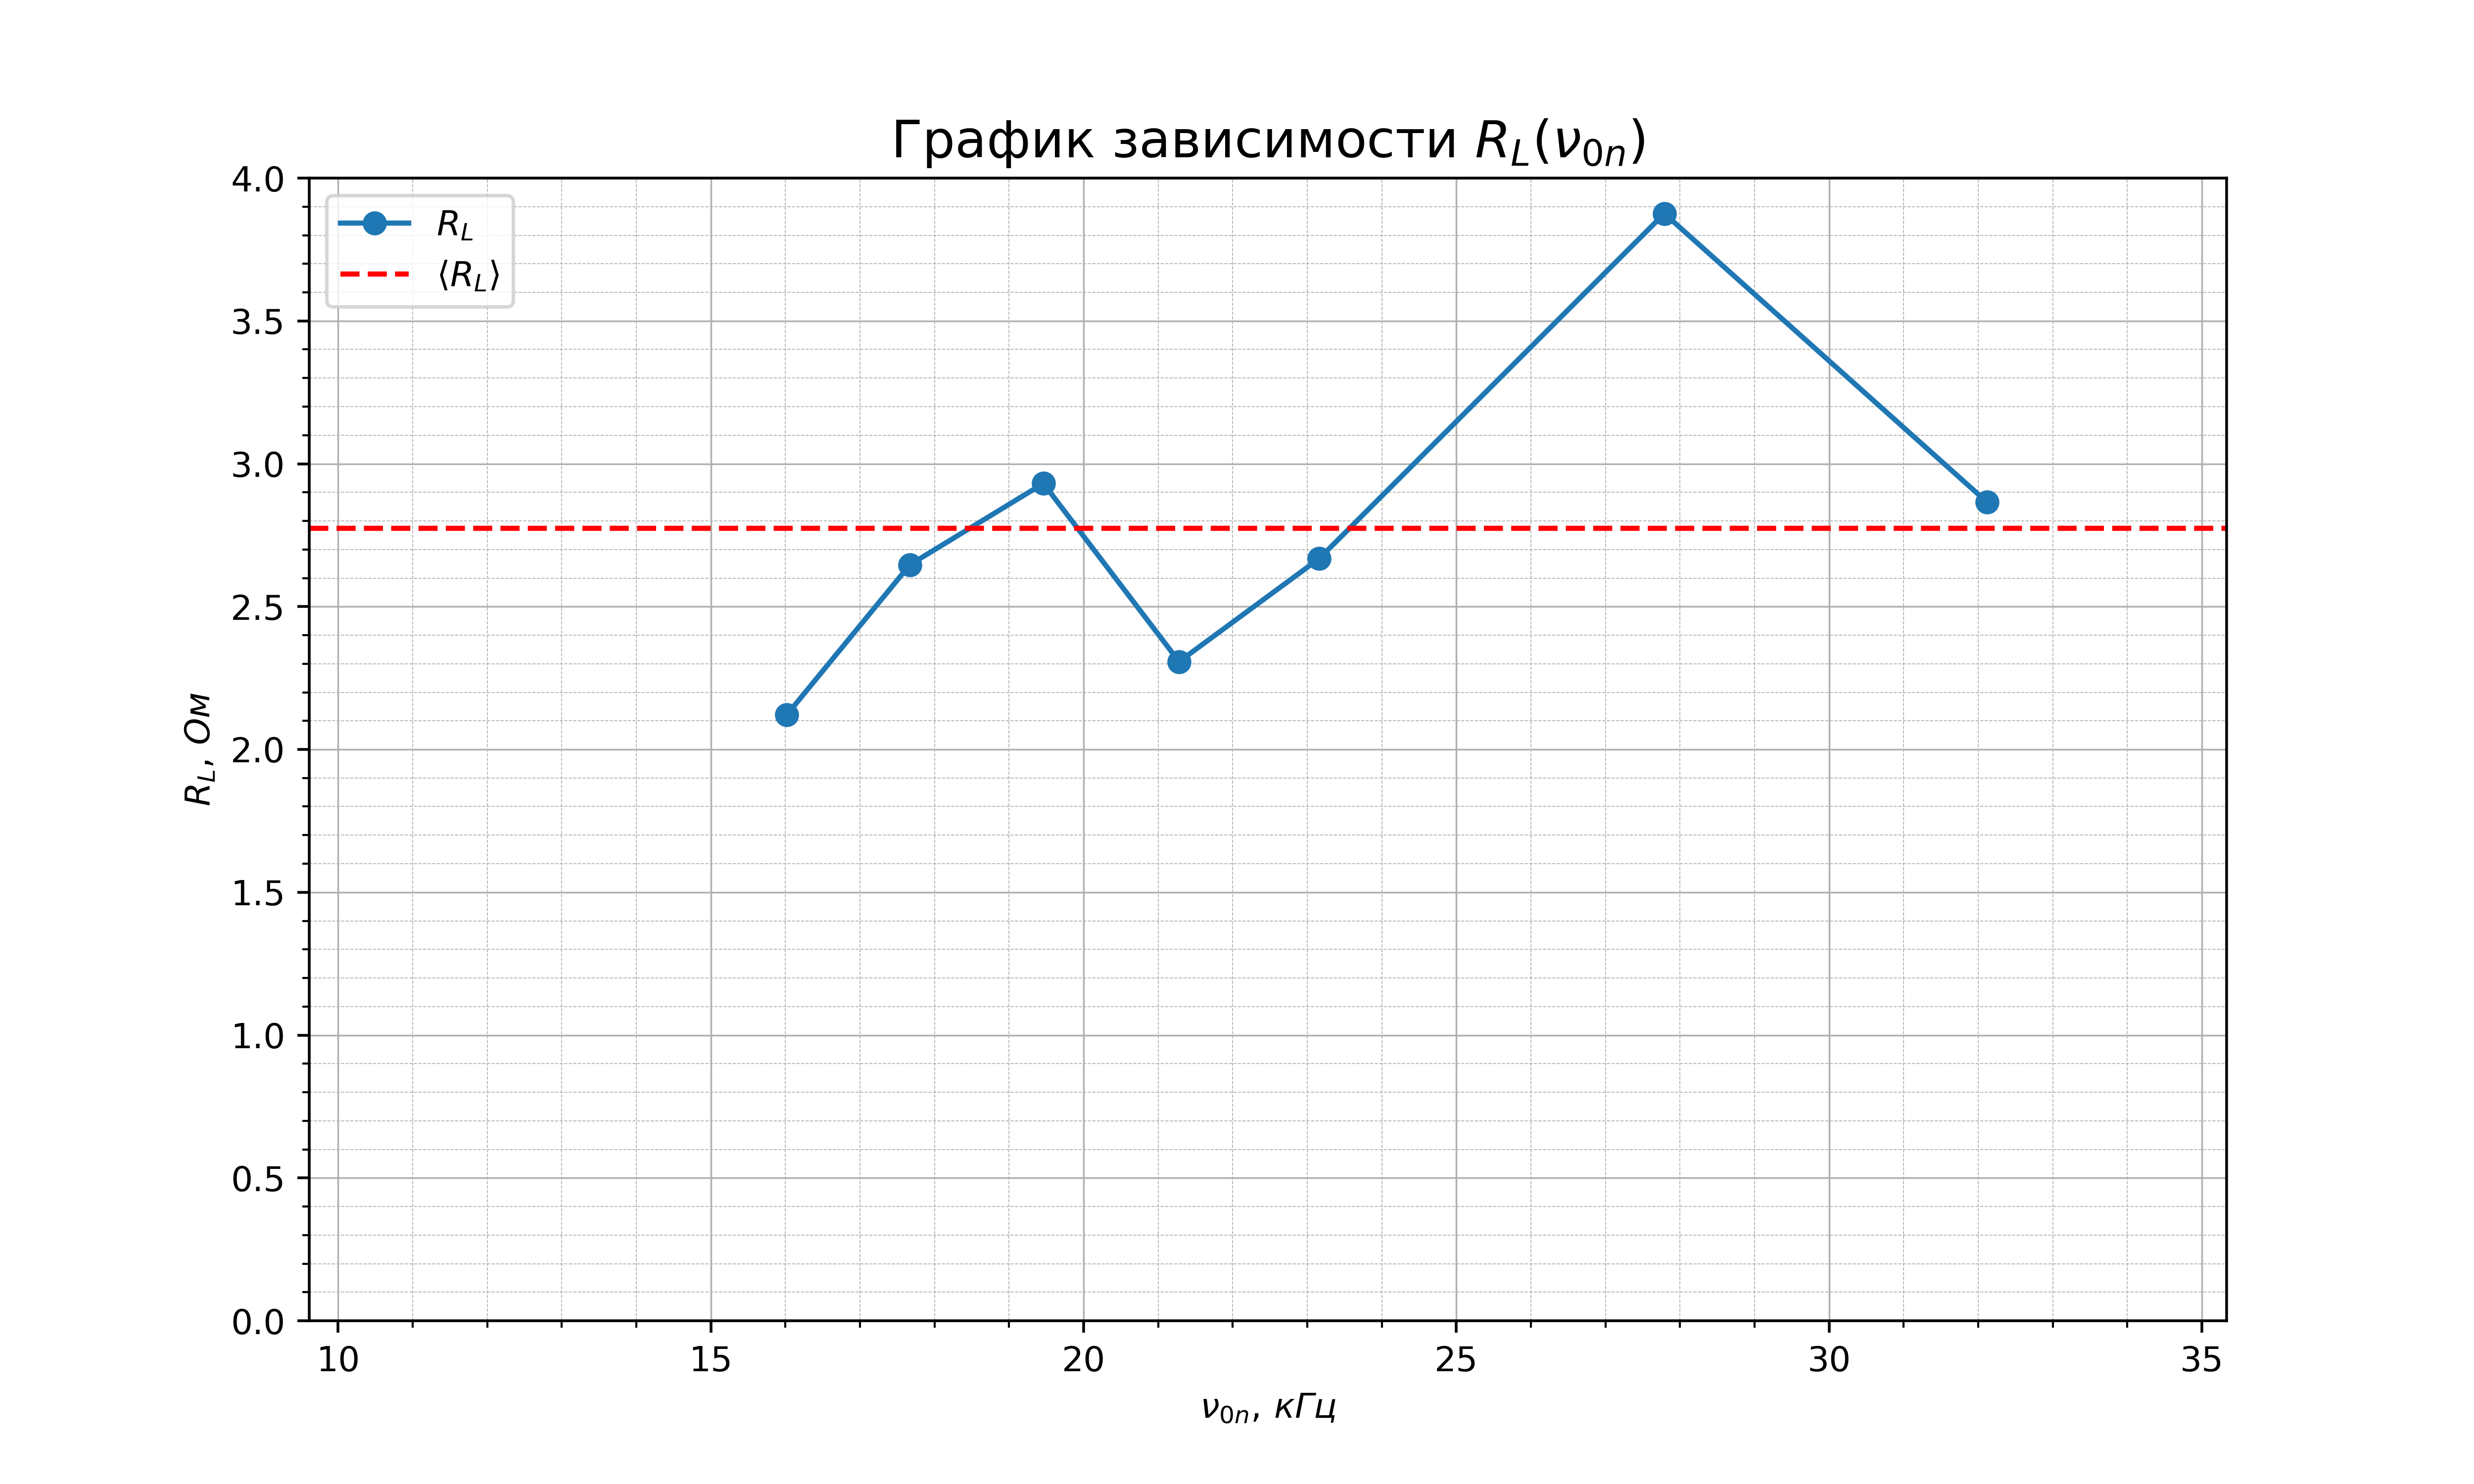
\includegraphics[scale=0.7]{3.2.3_4.png}
\end{center}
\caption{График зависимости активного сопротивления катушки $R_L$ от резонансной частоты контура $\nu_{0n}$}
\label{plot4}
\end{figure}

\newpage

\begin{wrapfigure}{l}{0.34\linewidth} 
	\begin{tikzpicture} [scale = 1.5, yshift=2pt]
		\draw  (0, 0) -- (0, 2.1);
		\draw (0, 0) -- (0, - 2.1);
		\draw  (0, 0) -- (2.5, 0);
		\draw [->] (0, 0) -- (0.75, 2) node[anchor=west] {$ \vec{I_C} $};
		\draw (0, 1.3) arc (60:0: 0.6);
			\draw (0.2,1.4) node {$ \varphi_C'$};
				\draw [->] (0, 0) -- (0.06, -2) node[anchor=west] {$ \vec{I_L} $};
			\draw (0, -1.3) arc (0:30: -0.4);
			\draw (0.15,-1.4) node {$ \delta$};
			\draw [->] (0, 0) -- (0.75, 0) node[anchor=south] {$ \vec{I} $};
			\draw [->] (0, 0) -- (1.75, -0.4) node[anchor=north] {$ \vec{U} $};
				\draw (1, 0) arc (30:0: 0.6);
					\draw (1.3, -0.1) node {$ \varphi_U$};
\end{tikzpicture}
\caption{Векторная диаграмма}
\end{wrapfigure}

Построим векторную диаграмму для контура с наименьшей добротностью, например, для $C_7$ с добротностью $Q_7 = 17$.

Посчитаем ток $ I = \dfrac{E}{R_1} = \dfrac{0,2}{1008} \approx 0,1 мА $. Его вектор равен сумме: $ \vec{I} = \vec{I_L} + \vec{I_C} $, причем $ \vec{I} $ расположен на оси абсцисс, а его компоненты расположены к нему под углами

\begin{equation}
\varphi_C = \dfrac{\pi}{2} - \dfrac{R + R_L}{\rho}, \quad \varphi_L = -\dfrac{\pi}{2} + \delta
\end{equation}

Здесь $ \delta \simeq 10^{-3}$ --- очень малый параметр установки, которым допустимо пренебречь при расчёте, однако можно изобразить для наглядности. Подсчитаем угол \newline $ \varphi_C' = \dfrac{R + R_L}{\rho} \approx 0,057 $. 

Аналогичный угол у напряжения $ \vec{U}: \varphi_U = - \dfrac{R + R_L}{\rho} $. Т.е. оно незначительно отклоняется от оси абсцисс на отрицательный угол.

\section{Обсуждение результатов и выводы}

В данной работе был исследован резонанс токов в параллельном колебательном контуре с изменяемой ёмкостью, были определены параметры контура, получены амплитудно-частотные и фазово-частотные характеристики контура при 2 различных значениях ёмкости конденсатора.  По графику АЧХ были определены добротности соответствующих контуров. Полученные значения:
$$ Q_1 = 29\pm1, \quad Q_7 = 16\pm1. $$
Также добротности были определены с помощью графика ФЧХ 2-мя способами. Значения, полученные 1-ым способом (по углу наклона прямой вблизи резонанса):
$$ Q_1 = 18\pm5, \quad Q_7 = 13\pm4. $$
Результат, полученный 2-ым способом (по расстоянию между y(-1/4) и y(1/4) по оси x):
$$ Q_1 = 17\pm1, \quad Q_7 = 13\pm1. $$
Значения добротности, рассчитанные теоретически:
$$ Q_1 = 30, \quad Q_7 = 17. $$
Результат, рассчитанный по АЧХ совпадает с теоретическим в пределах погрешности. Однако результаты, полученные при исследовании ФЧХ, совпадают по порядку, но существенно отличаются от рассчитанных теоретически. Это может быть связано с высокой погрешностью предложенного метода измерения сдвига фаз между $E$ и $U$ ввиду его сложности. Например, графики ФЧХ для обоих контуров не пересекают прямую $y = -1/4$, что говорит о наличии систематической погрешности измерений.

Также была определена зависимость активного сопротивления катушки $R_L$ от резонансной частоты $\nu_0$. Как видно из графика, $R_L$ возрастает с возрастанием частоты. Это может быть вызвано скин-эффектом. Резкое скачкообразное изменение значений $R_L$ может быть связано с изменением амплитуды ЭДС в процессе эксперимента.

\end{document}
